\documentclass[a4paper, 12pt]{article}
\usepackage[english]{babel}
\usepackage{amsmath}
\usepackage{graphicx}
\usepackage{caption}
\usepackage{subcaption}
\usepackage{placeins}
\usepackage[T1]{fontenc}
\usepackage[utf8]{inputenc}
\usepackage{floatrow}
\usepackage{amsmath}

\author{Maarten de Jonge \\
    Inge Becht}
\date{\today}
\title{Assignment 4\\ 
Slammin' and Jammin'}

\begin{document}
\maketitle
\section{Introduction}
In this exercise the use of the fastSLAM algorithm is explored for the NXT
legorobot. The idea of this algorithm is that the robot makes a map using no a
priori knowledge of the environment,
while at the same time determining its position in the map.
To use SLAM in general, two types of data need to be extracted. Firstly,
the robot needs to acquire landmarks from the
environment. These landsmarks in the case of this assignment are wall corners. To extract these
corners the same line extraction algorithm is used as in previous exercises (see assignment 2, 3 and 4). 
Secondly, the robot needs odometry to measure its distance to map the information found by the
sensors correctly. This idea has been explored in a
previous exercise as well (see assignment 1), but uses a noise distribution to
make the next position given the previous one a certaint measure of uncertainty.

Although the outline of the SLAM algorithm is already given, the implementation
of both odometry and landmark detection were left open as an exercise. The next
section will show what was implemented. After this different experiments were
done witht the FastSLAM
algorithm to show what paramets can be of a decisive factor when working with a
particle filter.


\section{The implementation}
The implemention of the slam algorithm was given ready made in MATLAB code, and
can be run using the function \texttt{control\_panel.m}. The functions in
\texttt{FitLine.m} and \texttt{predict\_odo} still need to be completed.

\texttt{FitLine.m} is part of the implementation to find the landmarks for the
SLAM algorithm, and as the name suggests the idea is to fit a line given the
cluster of input points. First the x,y position of the centroid is found by
calculating the mean of the points in the cloud. The orientation of $\alpha$ (
We work in pool coordinates) depens on nom and denom, as given in the exercise.
Now $r$ can be decided using:

\begin{align*}
    r = x cos \alpha + y sin \alpha
\end{align*}

The x and y values used here are the centroid x and y calculated earlier.
Fitline now return the parameters $\alpha$ and $r$ for a possible line in the
point cloud.

. The file \texttt{predict\_odo} tries to predict the new position of the robot
given some uncertainty in the covariancy matrix and the sensor values in the
wheel.
The x and y positions are calculated as follows:

\begin{align*}
    x_{t+1} = x_{t} + dr_n * cos(dth_n + \theta_t)\\
    y_{t+1} = y_{t} + dr_n * sin(dth_n + \theta_t)\\
\theta_{t+1} = \left\{ \begin{array}{rl}
 \theta_t + \theta_d + -2*\pi &\mbox{ if $\theta_t + \theta_d > \pi$} \\
 \theta_t + \theta_d + 2*\pi&\mbox{ otherwise}
\end{array} \right.
\end{align*}
where $x_{t+1}$ is the $x$ position of a particle on time $t+1$, $dr_n$ is a noise
parameter that adds uncertainty in the amount of distance driven between each
timestep, $dth_n$ is noise parameter for $\theta$ and $\theta_d$ the
difference in theta value between $\theta_t$  and $\theta_{t+1}$.
Using the \texttt{TEST\_ODO.m} file a test can be made of the performance of the
odometry prediction. In figure \ref{fig:odo_test} the resulting image given this test
can be admired. Unfortunately there was no baseline to test our results against,
except for the other students getting the same image as we did, as well as the
same value for the returned parameter \texttt{TOL\_JUMP} with a value of 10.5

\begin{figure}[!ht]
\centering
  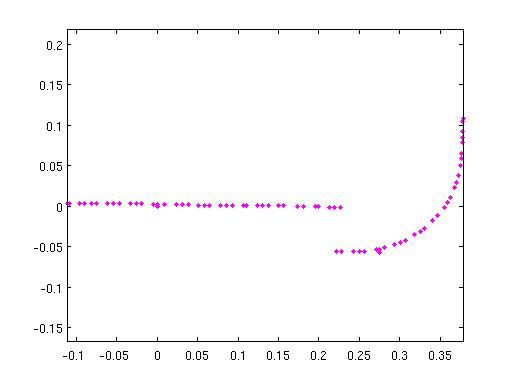
\includegraphics[width=0.5\textwidth]{Odo_test.jpg}
  \caption{Figure represented byt the \texttt{ODO\_TEST.m} file. } 
  \label{fig:odo_test}
\end{figure}


\section{Experiments}
Unfortunately we were unable to use the dataset recorded on the Mindstorms
robot, so all experiments were done on the provided sample logfile, in which the
robot moves forward for a bit through a hallway before turning left and
stopping. There the following parameters were available for testing:
\begin{itemize}
    \item the number of particles
    \item the odometry variance in distance (\texttt{sigmaX})
    \item the odometry variance in angle (\texttt{sigmaTH})
    \item the range finder variance in distance (\texttt{sigmaR})
    \item the range finder variance in angle (\texttt{sigmaB})
\end{itemize}

Table \ref{tbl:params} shows the combinations of parameters used. A set of
default parameters was given and has been used as the baseline. In each trial,
one parameter is changed in order to observe its contribution to the result.
While the algorithm goes through the data, each particle is drawn and remains
visible, showing the path traced by the robot. The detected features are also
drawn relative to each particle, leading to kind of a ``wall-cloud'' showing
where a wall might be along with the certainty.

The script used for the experiments can be found in \texttt{control\_panel.m} on
the ``experiments'' branch of the Git repository.

\begin{table}[htbp]
    \begin{tabular}{|l|l|l|l|l|}
    \hline
    sigmaX & sigmaTH & sigmaR & sigmaB & particles \\
    \hline
    0.003  & 0.02    & 0.01   & 0.01   & 200       \\
    0.05   & 0.02    & 0.01   & 0.01   & 200       \\
    0.1    & 0.02    & 0.01   & 0.01   & 200       \\
    0.003  & 0.1     & 0.01   & 0.01   & 200       \\
    0.003  & 0.5     & 0.01   & 0.01   & 200       \\
    0.003  & 0.02    & 0.1    & 0.01   & 200       \\
    0.003  & 0.02    & 0.5    & 0.01   & 200       \\
    0.003  & 0.02    & 0.01   & 0.1    & 200       \\
    0.003  & 0.02    & 0.01   & 0.5    & 200       \\
    0.003  & 0.02    & 0.01   & 0.01   & 10        \\
    0.003  & 0.02    & 0.01   & 0.01   & 1000      \\
    \hline
    \end{tabular}
    \caption{The parameters used for the experiments. Each row represents one
    trial.}
    \label{tbl:params}
\end{table}

\section{Results}
Only using a logfile of an unknown environment makes it hard to quantify the
output of the algorithm. The final picture output by the algorithm is taken as
the result. The left half shows the the locations of every particle over the
course of the algorithm in red, and the detected walls in black. The right half
shows the sensor input in the last frame, and is irrelevant to the performance
of the algorithm. The results are show in figures \ref{fig:results1} and
\ref{fig:results2}.

\begin{figure}
    \centering
    \begin{subfigure}[b]{0.4\textwidth}
        \centering
        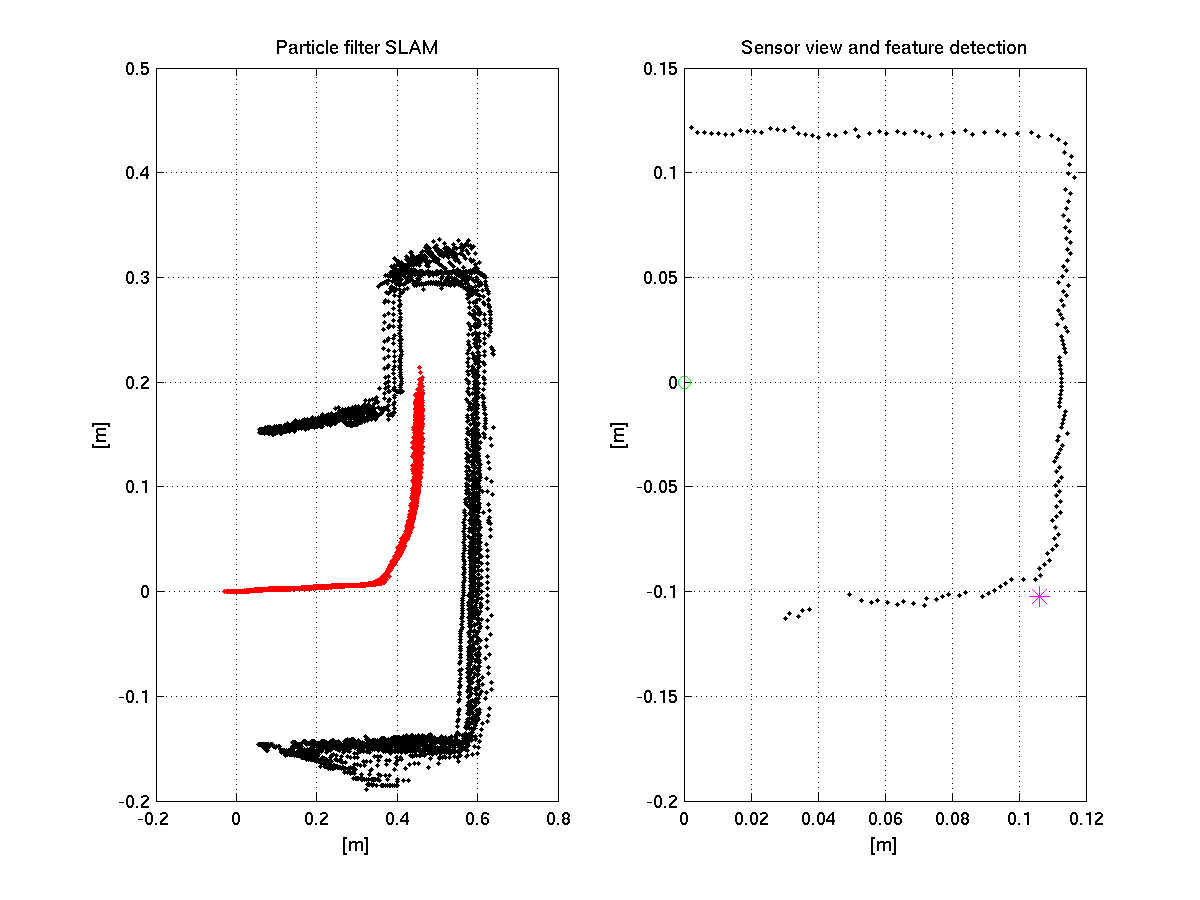
\includegraphics[width=\textwidth]{fig/default.png}
        \caption{the default parameters}
    \end{subfigure}

    \begin{subfigure}[b]{0.4\textwidth}
        \centering
        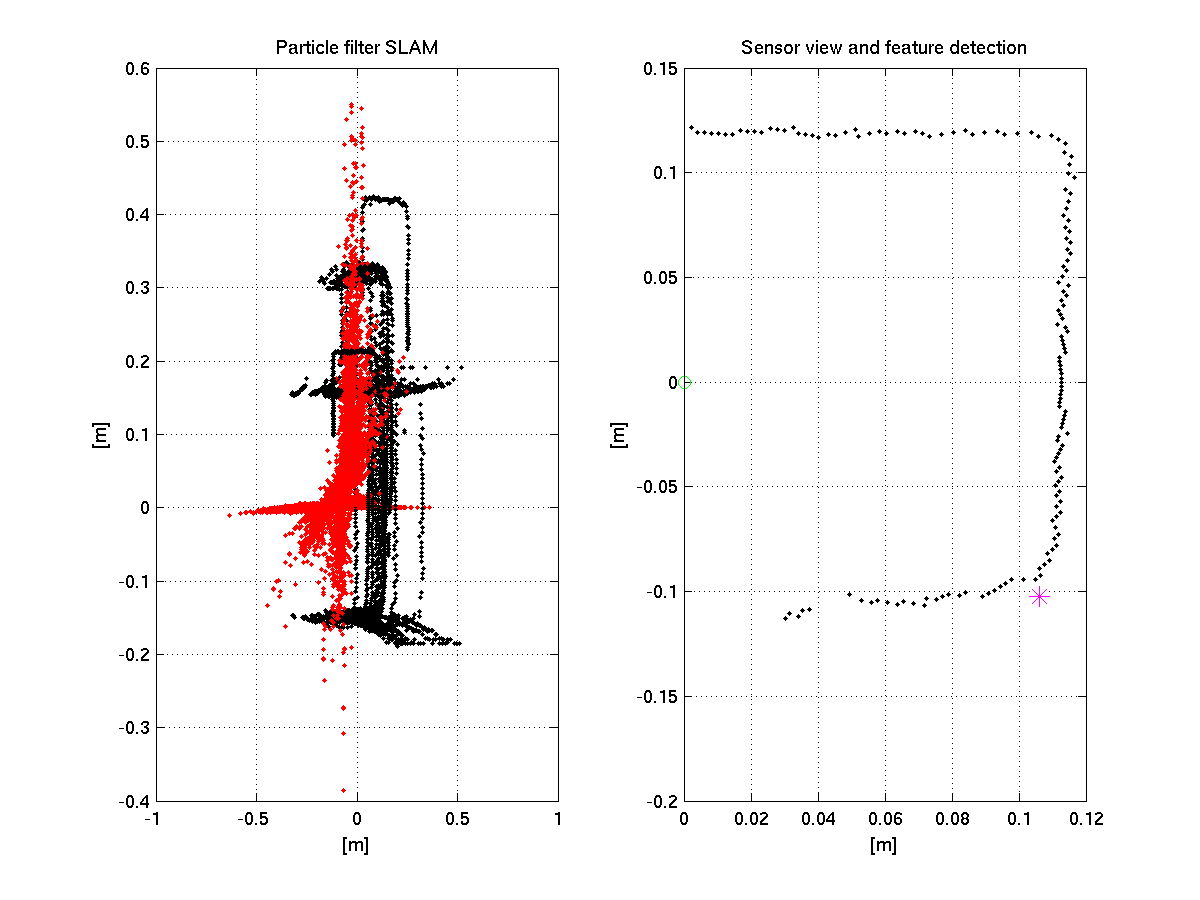
\includegraphics[width=\textwidth]{{fig/sigmaX_0.05}.png}
        \caption{\texttt{sigmaX} at 0.05}
    \end{subfigure}
    ~ 
    \begin{subfigure}[b]{0.4\textwidth}
        \centering
        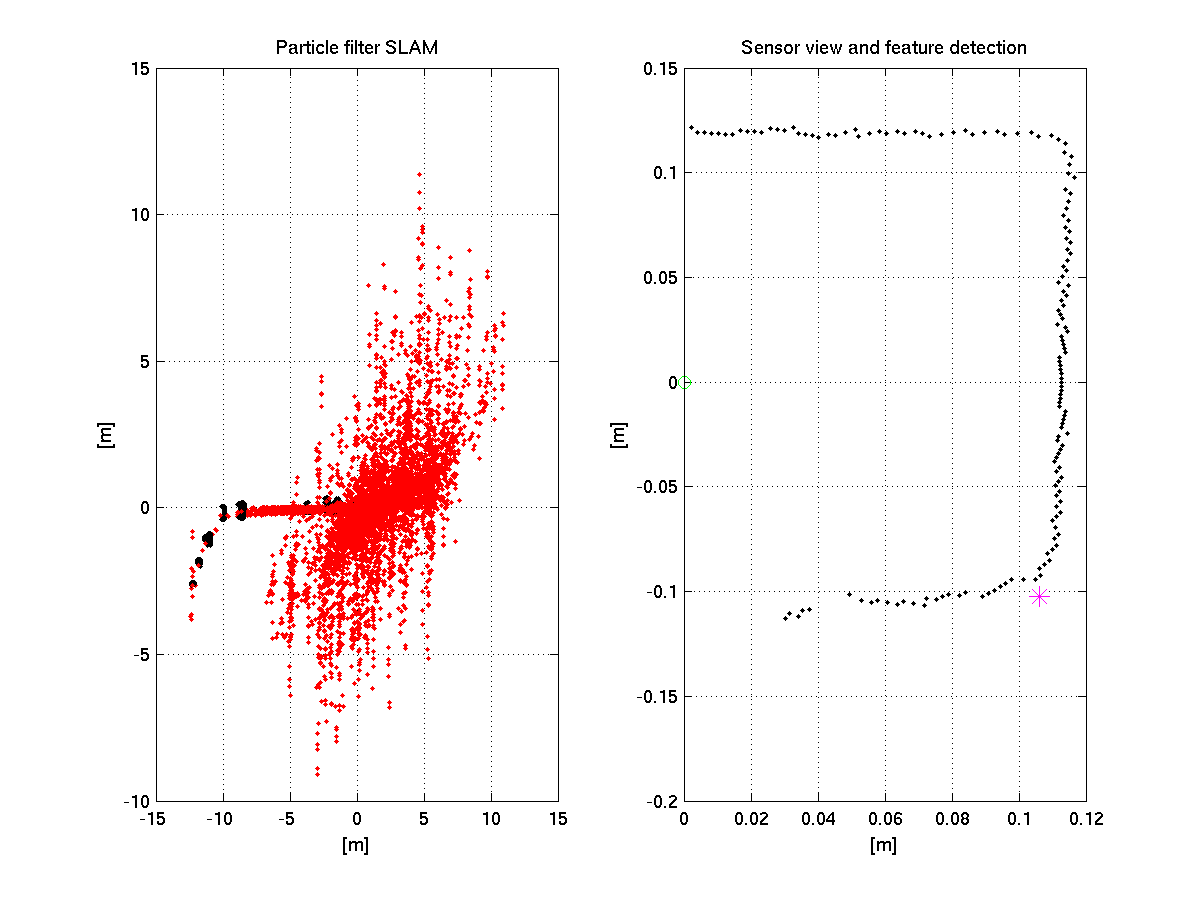
\includegraphics[width=\textwidth]{fig/sigmaX_1.png}
        \caption{\texttt{sigmaX} at 1}
    \end{subfigure}

    \begin{subfigure}[b]{0.4\textwidth}
        \centering
        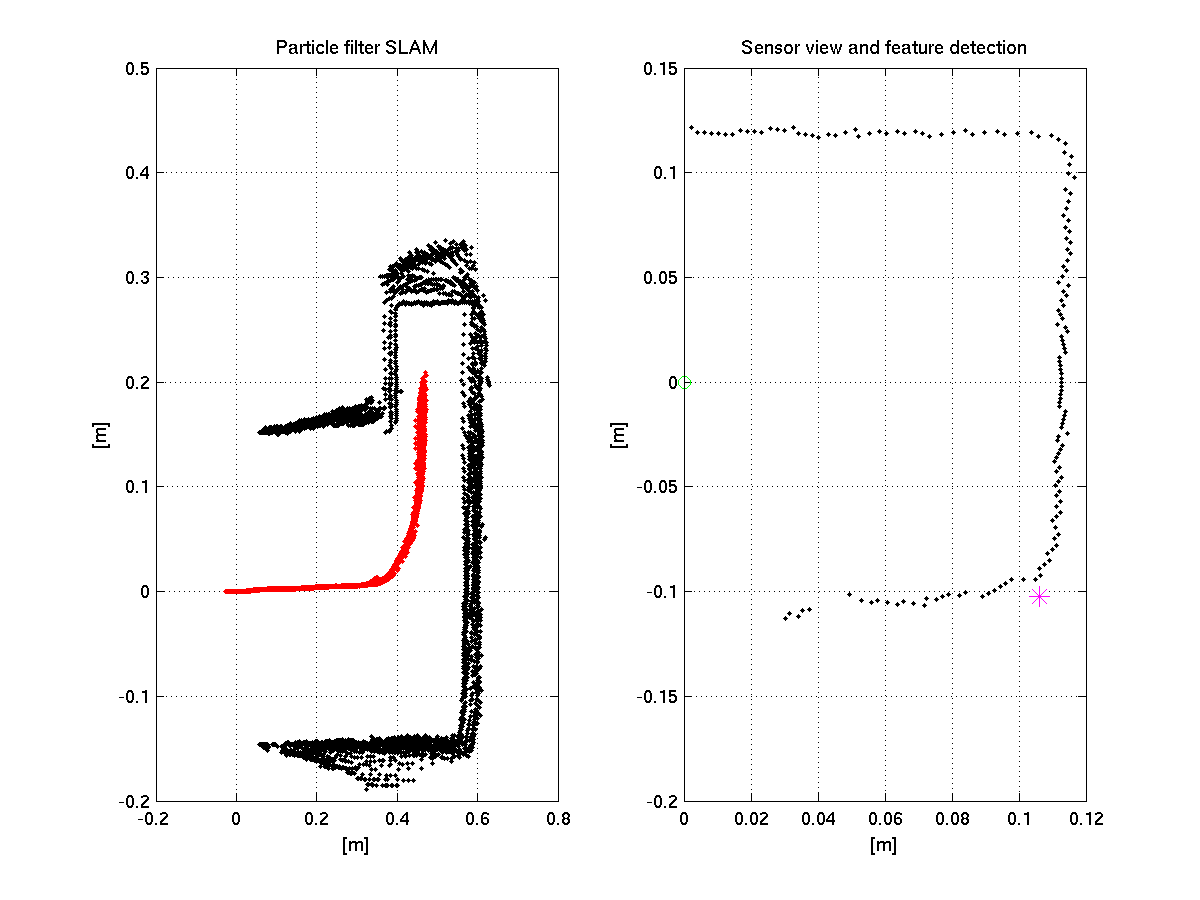
\includegraphics[width=\textwidth]{{fig/sigmaTH_0.1}.png}
        \caption{\texttt{sigmaTH} at 0.1}
    \end{subfigure}
    ~ 
    \begin{subfigure}[b]{0.4\textwidth}
        \centering
    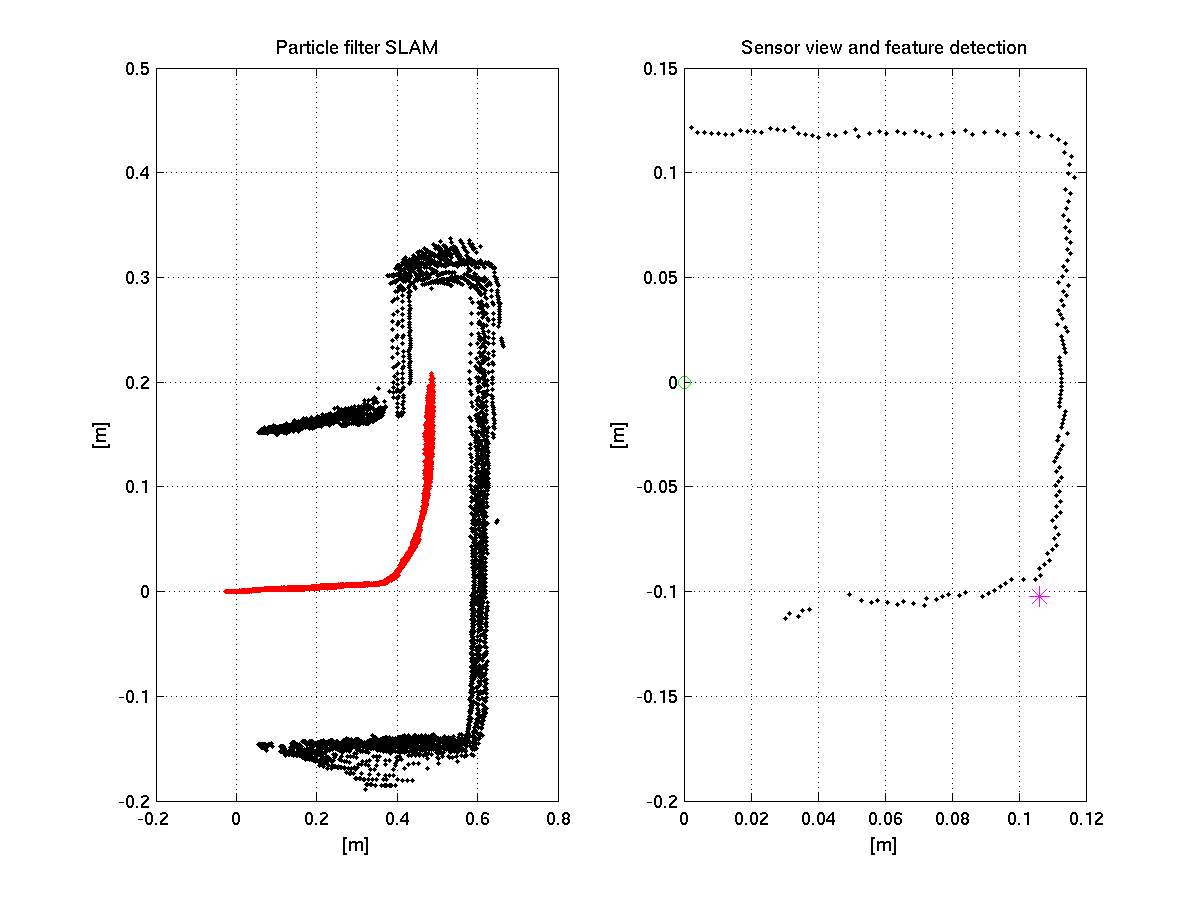
\includegraphics[width=\textwidth]{{fig/sigmaTH_0.5}.png}
        \caption{\texttt{sigmaTH} at 0.5}
    \end{subfigure}

    \begin{subfigure}[b]{0.4\textwidth}
        \centering
        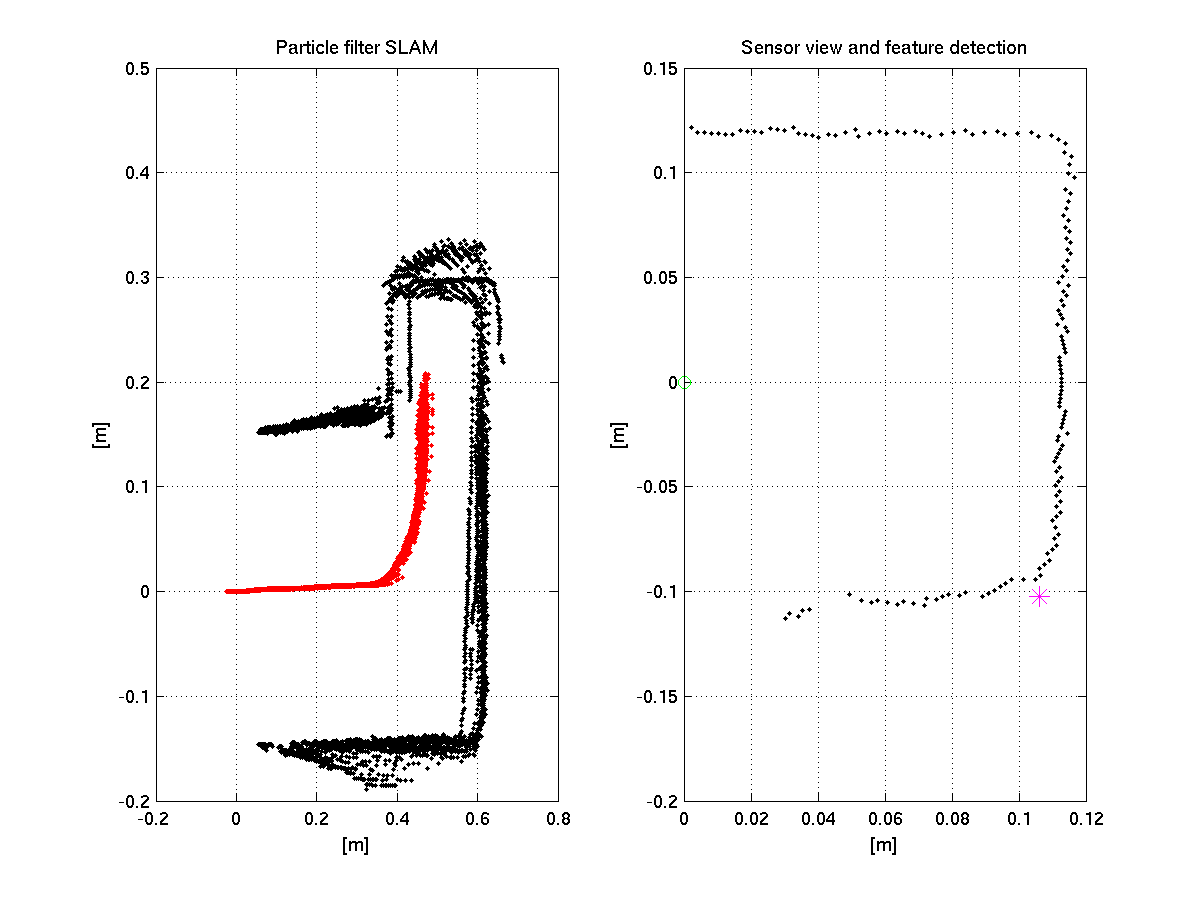
\includegraphics[width=\textwidth]{{fig/sigmaRs_0.1}.png}
        \caption{\texttt{sigmaR} at 0.1}
    \end{subfigure}
    ~ 
    \begin{subfigure}[b]{0.4\textwidth}
        \centering
    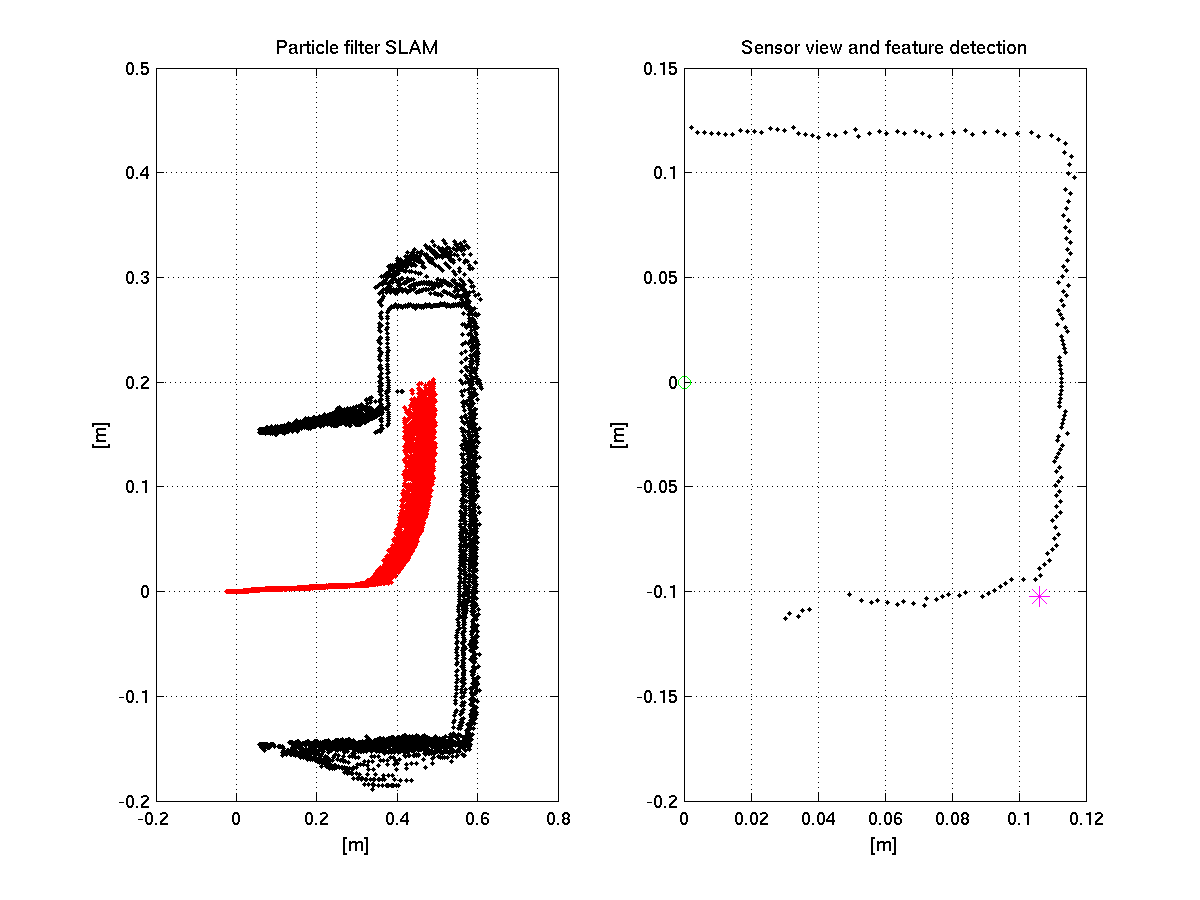
\includegraphics[width=\textwidth]{{fig/sigmaRs_0.5}.png}
        \caption{\texttt{sigmaR} at 0.5}
    \end{subfigure}
    \caption{SLAM results, part 1}
    \label{fig:results1}
\end{figure}

\begin{figure}
    \centering
    \begin{subfigure}[b]{0.4\textwidth}
        \centering
        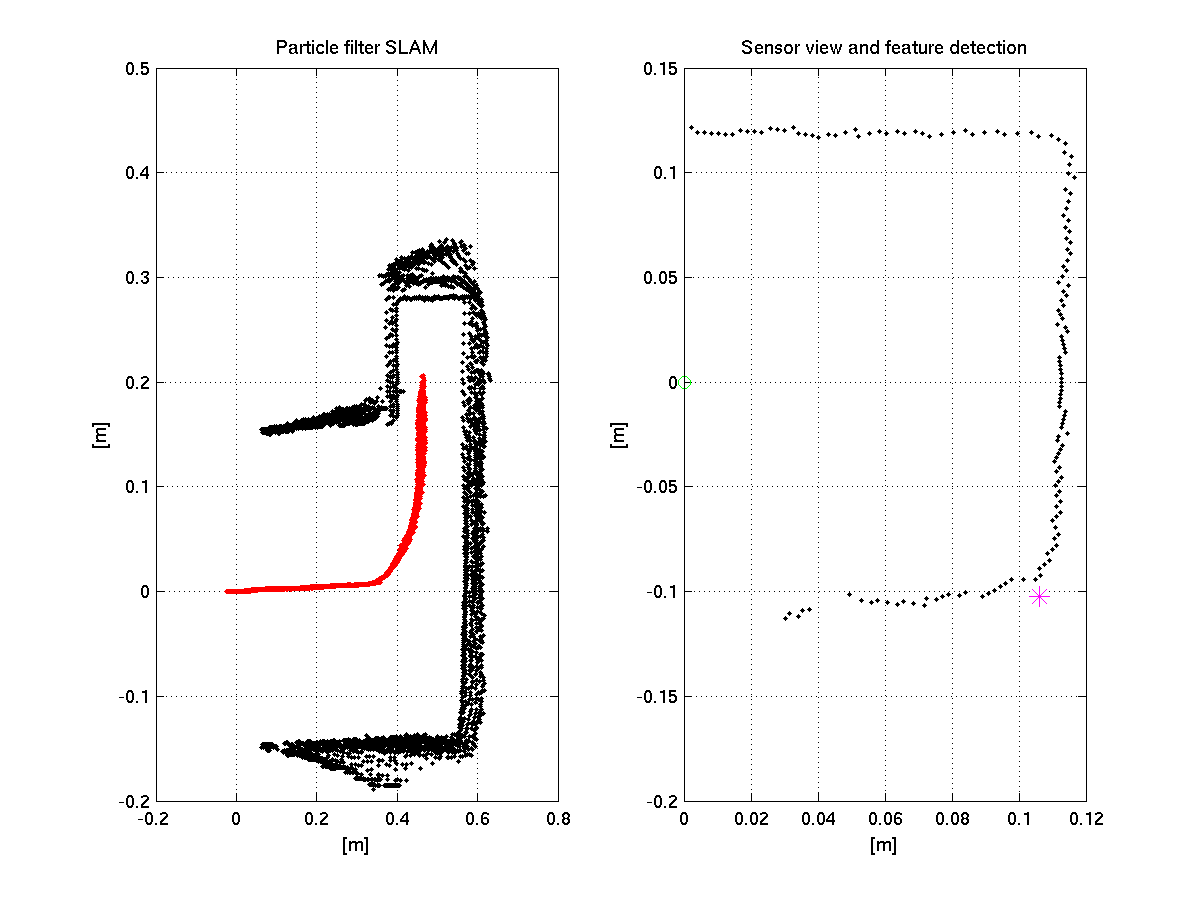
\includegraphics[width=\textwidth]{{fig/sigmaBs_0.1}.png}
        \caption{\texttt{sigmaB} at 0.1}
    \end{subfigure}
    ~ 
    \begin{subfigure}[b]{0.4\textwidth}
        \centering
    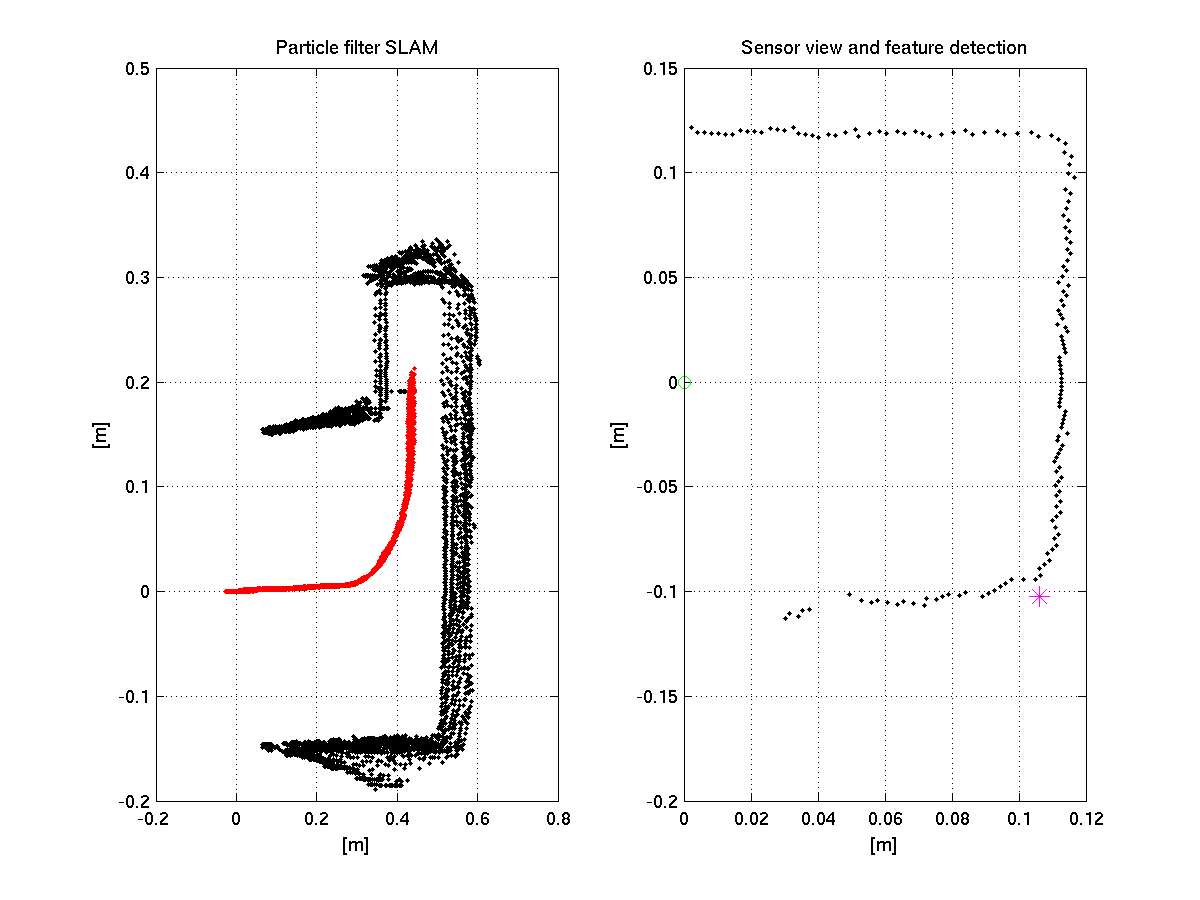
\includegraphics[width=\textwidth]{{fig/sigmaBs_0.5}.png}
        \caption{\texttt{sigmaB} at 0.5}
    \end{subfigure}
    
    \begin{subfigure}[b]{0.4\textwidth}
        \centering
        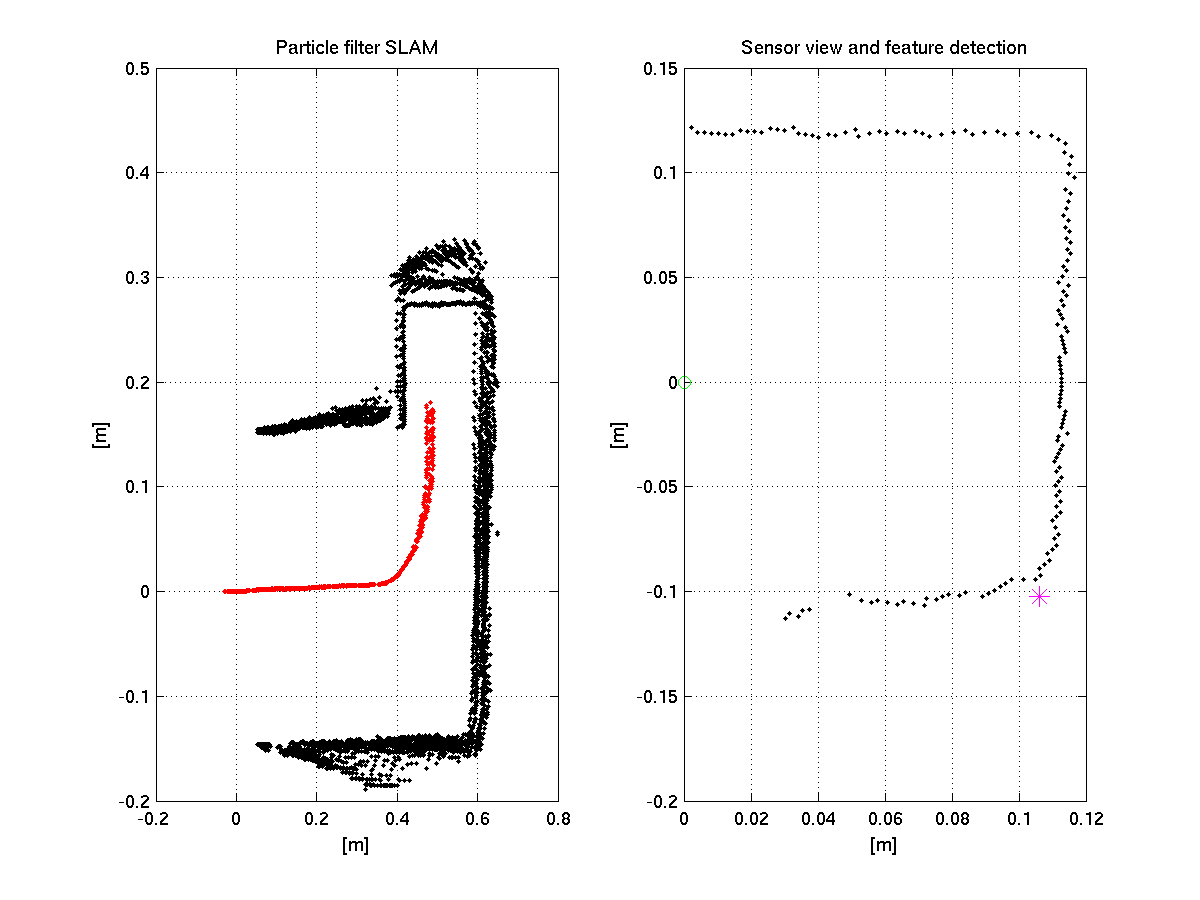
\includegraphics[width=\textwidth]{{fig/particles_10}.png}
        \caption{particles at 10}
    \end{subfigure}
    ~ 
    \begin{subfigure}[b]{0.4\textwidth}
        \centering
    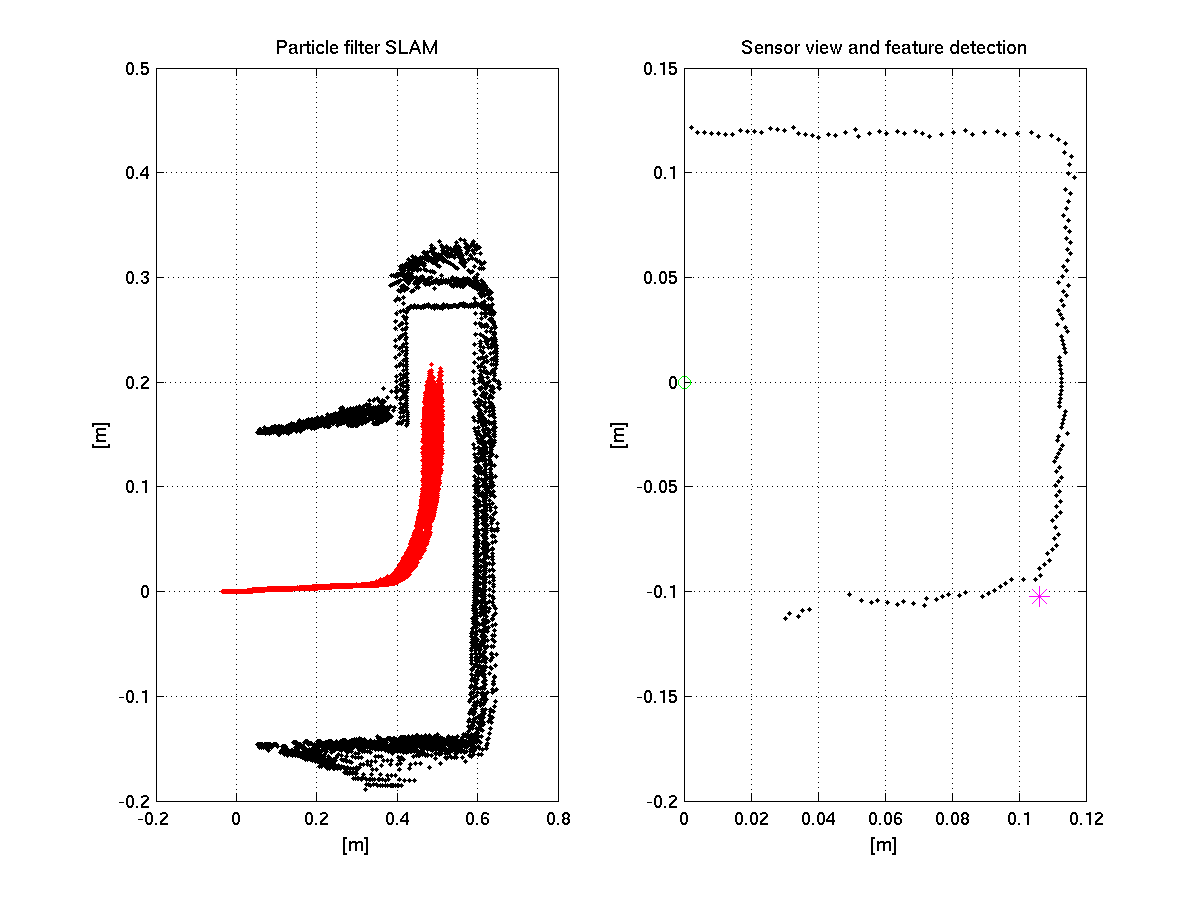
\includegraphics[width=\textwidth]{{fig/particles_1000}.png}
        \caption{particles at 1000}
    \end{subfigure}

    \caption{SLAM results, part 2}
    \label{fig:results2}
\end{figure}

The default parameters lead to a pretty certain localisation, and not much
uncertainty in the mapping. Raising the odometry's distance uncertainty leads
has a dramatic effect on the end result, rendering it essentially unusable. The
angle variance appears less dramatic, only slightly increasing the uncertainty
of the map with no visible influence on the certainty of localisation. In
hindsight, parameters tested might have been suboptimal. Because the distance
variance is specified in meters and the angle variance in degrees, the chosen
parameters are biased in favor the rotation; a 1 meter inaccuracy is far more
dramatic than an inaccuracy of 1 degree.

The distance variance in the range finger has a notable effect on the certainty
of the robot's location; the path is clearly thicker, with more ambiguity as to
the distance of the robot to the wall. The angle variance mainly seems to make
the location of the walls slightly more uncertain, without much effect in
regards to the localisation.

Surprisingly, the number of particles does little except for deciding the
thickness of the red line, which probably means the full extent of the
uncertainty is insufficiently represented with only 10 particles, as one could
except. In either case, the mapping and localisation are practically the same.
Perhaps this is due to the short path travelled by the robot; the number of
particles might have a far stronger influence on longer, non-trivial journeys.


\end{document}
